\documentclass[border=2mm]{standalone}
\usepackage{tikz}
\begin{document}
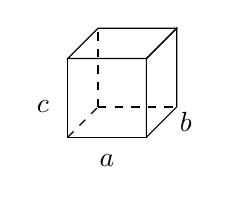
\begin{tikzpicture}
    \pgfmathsetmacro{\cubex}{1}
    \pgfmathsetmacro{\cubey}{1}
    \pgfmathsetmacro{\cubez}{1}
    \draw (0,0,0) -- ++(-\cubex,0,0) -- ++(0,-\cubey,0) -- ++(\cubex,0,0) -- cycle;
    \draw (0,0,0) -- ++(0,0,-\cubez) -- ++(0,-\cubey,0) -- ++(0,0,\cubez) -- cycle;
    \draw (0,0,0) -- ++(-\cubex,0,0) -- ++(0,0,-\cubez) -- ++(\cubex,0,0) -- cycle;
    \draw[dashed] (-\cubex,-\cubey,0) -- (-\cubex,-\cubey,-\cubez);
    \draw[dashed] (-\cubex,-\cubey,-\cubez) -- (0, -\cubey,-\cubez);
    \draw[dashed] (-\cubex,-\cubey,-\cubez) -- (0, -\cubey,-\cubez);
    \draw[dashed] (-\cubex,-\cubey,-\cubez) -- (-\cubex, 0,-\cubez);
    \node at(-0.5,-1.3,0) {$a$};
    \node at(0.5,-0.8,0) {$b$};
    \node at(-1.7,-1,-1) {$c$};
\end{tikzpicture}
\end{document}